\documentclass[]{article}
\usepackage{lmodern}
\usepackage{amssymb,amsmath}
\usepackage{ifxetex,ifluatex}
\usepackage{fixltx2e} % provides \textsubscript
\ifnum 0\ifxetex 1\fi\ifluatex 1\fi=0 % if pdftex
  \usepackage[T1]{fontenc}
  \usepackage[utf8]{inputenc}
\else % if luatex or xelatex
  \ifxetex
    \usepackage{mathspec}
  \else
    \usepackage{fontspec}
  \fi
  \defaultfontfeatures{Ligatures=TeX,Scale=MatchLowercase}
\fi
% use upquote if available, for straight quotes in verbatim environments
\IfFileExists{upquote.sty}{\usepackage{upquote}}{}
% use microtype if available
\IfFileExists{microtype.sty}{%
\usepackage{microtype}
\UseMicrotypeSet[protrusion]{basicmath} % disable protrusion for tt fonts
}{}
\usepackage[margin=1in]{geometry}
\usepackage{hyperref}
\hypersetup{unicode=true,
            pdftitle={Hello R Markdown},
            pdfborder={0 0 0},
            breaklinks=true}
\urlstyle{same}  % don't use monospace font for urls
\usepackage{color}
\usepackage{fancyvrb}
\newcommand{\VerbBar}{|}
\newcommand{\VERB}{\Verb[commandchars=\\\{\}]}
\DefineVerbatimEnvironment{Highlighting}{Verbatim}{commandchars=\\\{\}}
% Add ',fontsize=\small' for more characters per line
\usepackage{framed}
\definecolor{shadecolor}{RGB}{248,248,248}
\newenvironment{Shaded}{\begin{snugshade}}{\end{snugshade}}
\newcommand{\KeywordTok}[1]{\textcolor[rgb]{0.13,0.29,0.53}{\textbf{#1}}}
\newcommand{\DataTypeTok}[1]{\textcolor[rgb]{0.13,0.29,0.53}{#1}}
\newcommand{\DecValTok}[1]{\textcolor[rgb]{0.00,0.00,0.81}{#1}}
\newcommand{\BaseNTok}[1]{\textcolor[rgb]{0.00,0.00,0.81}{#1}}
\newcommand{\FloatTok}[1]{\textcolor[rgb]{0.00,0.00,0.81}{#1}}
\newcommand{\ConstantTok}[1]{\textcolor[rgb]{0.00,0.00,0.00}{#1}}
\newcommand{\CharTok}[1]{\textcolor[rgb]{0.31,0.60,0.02}{#1}}
\newcommand{\SpecialCharTok}[1]{\textcolor[rgb]{0.00,0.00,0.00}{#1}}
\newcommand{\StringTok}[1]{\textcolor[rgb]{0.31,0.60,0.02}{#1}}
\newcommand{\VerbatimStringTok}[1]{\textcolor[rgb]{0.31,0.60,0.02}{#1}}
\newcommand{\SpecialStringTok}[1]{\textcolor[rgb]{0.31,0.60,0.02}{#1}}
\newcommand{\ImportTok}[1]{#1}
\newcommand{\CommentTok}[1]{\textcolor[rgb]{0.56,0.35,0.01}{\textit{#1}}}
\newcommand{\DocumentationTok}[1]{\textcolor[rgb]{0.56,0.35,0.01}{\textbf{\textit{#1}}}}
\newcommand{\AnnotationTok}[1]{\textcolor[rgb]{0.56,0.35,0.01}{\textbf{\textit{#1}}}}
\newcommand{\CommentVarTok}[1]{\textcolor[rgb]{0.56,0.35,0.01}{\textbf{\textit{#1}}}}
\newcommand{\OtherTok}[1]{\textcolor[rgb]{0.56,0.35,0.01}{#1}}
\newcommand{\FunctionTok}[1]{\textcolor[rgb]{0.00,0.00,0.00}{#1}}
\newcommand{\VariableTok}[1]{\textcolor[rgb]{0.00,0.00,0.00}{#1}}
\newcommand{\ControlFlowTok}[1]{\textcolor[rgb]{0.13,0.29,0.53}{\textbf{#1}}}
\newcommand{\OperatorTok}[1]{\textcolor[rgb]{0.81,0.36,0.00}{\textbf{#1}}}
\newcommand{\BuiltInTok}[1]{#1}
\newcommand{\ExtensionTok}[1]{#1}
\newcommand{\PreprocessorTok}[1]{\textcolor[rgb]{0.56,0.35,0.01}{\textit{#1}}}
\newcommand{\AttributeTok}[1]{\textcolor[rgb]{0.77,0.63,0.00}{#1}}
\newcommand{\RegionMarkerTok}[1]{#1}
\newcommand{\InformationTok}[1]{\textcolor[rgb]{0.56,0.35,0.01}{\textbf{\textit{#1}}}}
\newcommand{\WarningTok}[1]{\textcolor[rgb]{0.56,0.35,0.01}{\textbf{\textit{#1}}}}
\newcommand{\AlertTok}[1]{\textcolor[rgb]{0.94,0.16,0.16}{#1}}
\newcommand{\ErrorTok}[1]{\textcolor[rgb]{0.64,0.00,0.00}{\textbf{#1}}}
\newcommand{\NormalTok}[1]{#1}
\usepackage{graphicx,grffile}
\makeatletter
\def\maxwidth{\ifdim\Gin@nat@width>\linewidth\linewidth\else\Gin@nat@width\fi}
\def\maxheight{\ifdim\Gin@nat@height>\textheight\textheight\else\Gin@nat@height\fi}
\makeatother
% Scale images if necessary, so that they will not overflow the page
% margins by default, and it is still possible to overwrite the defaults
% using explicit options in \includegraphics[width, height, ...]{}
\setkeys{Gin}{width=\maxwidth,height=\maxheight,keepaspectratio}
\IfFileExists{parskip.sty}{%
\usepackage{parskip}
}{% else
\setlength{\parindent}{0pt}
\setlength{\parskip}{6pt plus 2pt minus 1pt}
}
\setlength{\emergencystretch}{3em}  % prevent overfull lines
\providecommand{\tightlist}{%
  \setlength{\itemsep}{0pt}\setlength{\parskip}{0pt}}
\setcounter{secnumdepth}{0}
% Redefines (sub)paragraphs to behave more like sections
\ifx\paragraph\undefined\else
\let\oldparagraph\paragraph
\renewcommand{\paragraph}[1]{\oldparagraph{#1}\mbox{}}
\fi
\ifx\subparagraph\undefined\else
\let\oldsubparagraph\subparagraph
\renewcommand{\subparagraph}[1]{\oldsubparagraph{#1}\mbox{}}
\fi

%%% Use protect on footnotes to avoid problems with footnotes in titles
\let\rmarkdownfootnote\footnote%
\def\footnote{\protect\rmarkdownfootnote}

%%% Change title format to be more compact
\usepackage{titling}

% Create subtitle command for use in maketitle
\newcommand{\subtitle}[1]{
  \posttitle{
    \begin{center}\large#1\end{center}
    }
}

\setlength{\droptitle}{-2em}

  \title{Hello R Markdown}
    \pretitle{\vspace{\droptitle}\centering\huge}
  \posttitle{\par}
    \author{}
    \preauthor{}\postauthor{}
    \date{}
    \predate{}\postdate{}
  

\begin{document}
\maketitle

This is a paragraph in a n R mMarkdown document.

Below is a code chunk:

\begin{Shaded}
\begin{Highlighting}[]
\NormalTok{fit<-}\StringTok{ }\KeywordTok{lm}\NormalTok{(dist }\OperatorTok{~}\StringTok{ }\NormalTok{speed, }\DataTypeTok{data =}\NormalTok{ cars)}
\NormalTok{b<-}\StringTok{ }\KeywordTok{coef}\NormalTok{(fit)}
\KeywordTok{plot}\NormalTok{(cars)}
\KeywordTok{abline}\NormalTok{(fit)}
\end{Highlighting}
\end{Shaded}

\includegraphics{day11_selflearn_files/figure-latex/unnamed-chunk-1-1.pdf}

The slope of the regression is 3.9324088.

To mark text as \texttt{inline\ code}, use a pair of backticks, e.g.,
\texttt{code}. To include n literal bacxkticks, use at least n+1
backticks outside, e.g., you can use four backticks to preservie three
backtick inside:
\texttt{code\textasciigrave{}\textasciigrave{}\textasciigrave{}\textasciigrave{}\textasciigrave{},\ which\ is\ rendered\ as\ \textasciigrave{}\textasciigrave{}\textasciigrave{}code}.

Hyperlinks are created using the syntax \href{link}{text}, e.g.,
\href{https://www.rstudio.com}{RStudio}. The syntax for images is
similiar: just add an exclamation mark, e.g.,

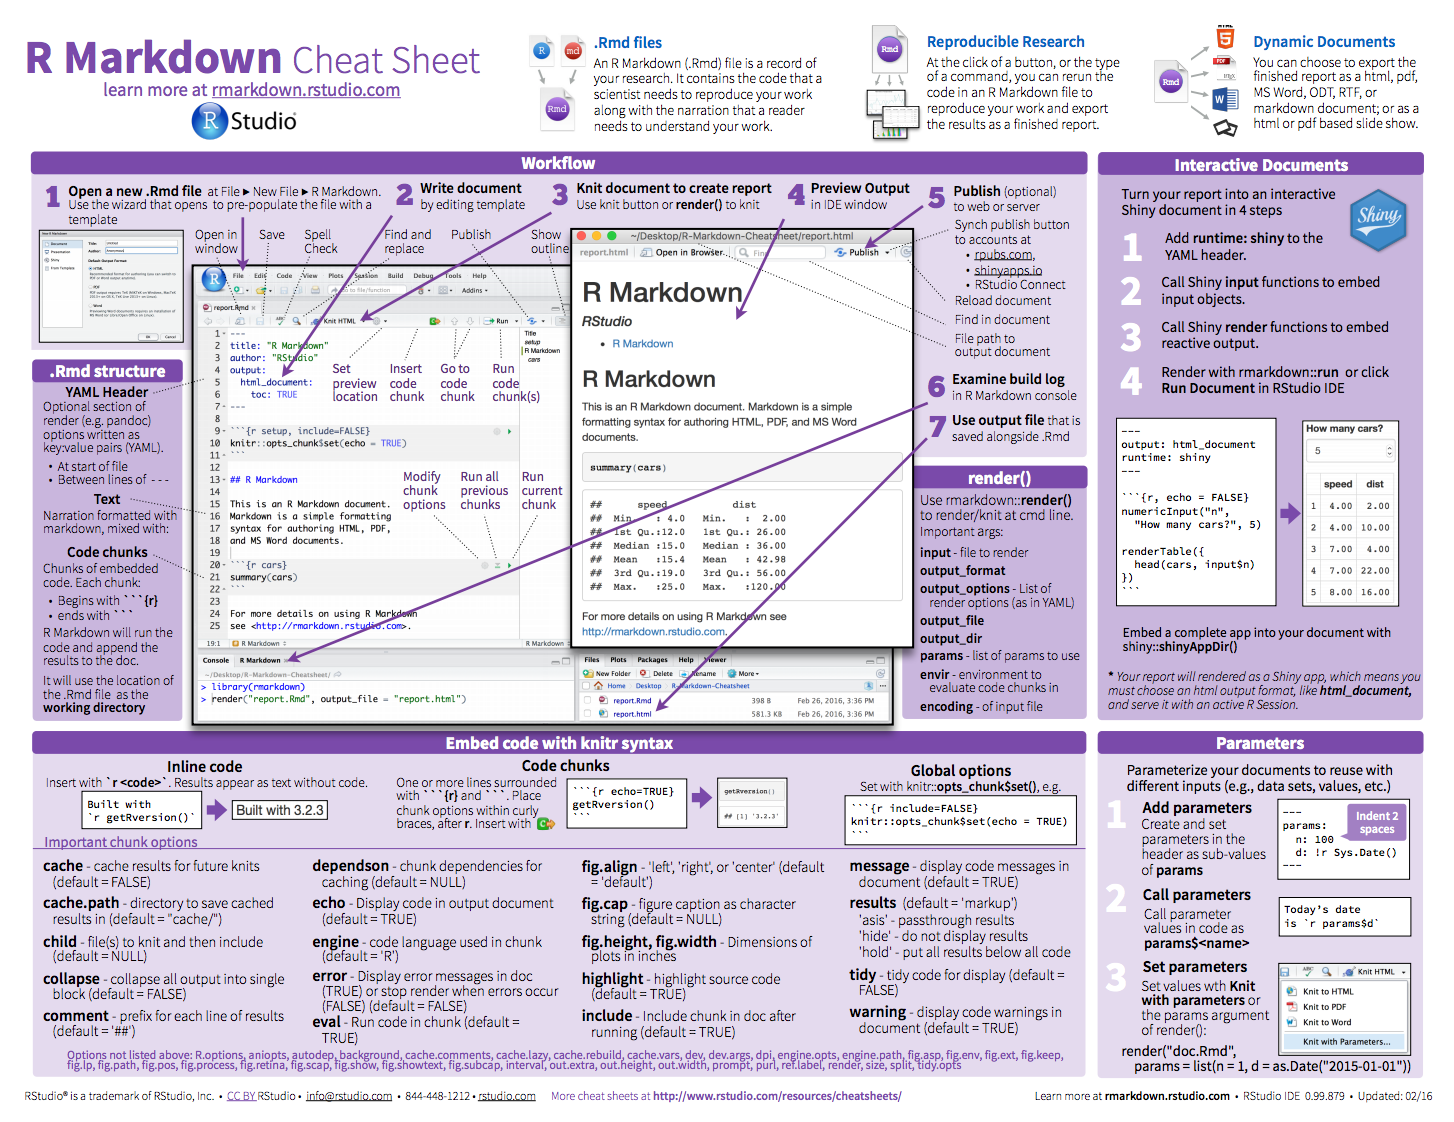
\includegraphics{C:/Jian/RStudio/ Conference/myrepo/myrepo/figs/rmarkdown.png}.

Footnotes are put inside the square brackets after a caret \footnote{Here
  is the first footnote}, e.g., Hello Jasmine\footnote{A nice place for
  chill and relax}.

There are multiple ways to insert citations, and we recommend that you
use BibTex databases, because they work better wwhen the output format
is LaTeX/PDF. Section 2.8 of Xie (2016) has explained the details. The
key idea is that when you have a BibTex databse (a plain-text file with
the conventional filename extension .bib) that contains entries like:

\begin{Shaded}
\begin{Highlighting}[]
\OperatorTok{@}\NormalTok{Manual\{R}\OperatorTok{-}\NormalTok{base,}
\NormalTok{  title=\{R}\OperatorTok{:}\StringTok{ }\NormalTok{A Language and Environment }\ControlFlowTok{for}\NormalTok{ Statistical Computing\},}
\NormalTok{  author=\{\{PR Core Team\}\},}
\NormalTok{  organization=\{R Foundation }\ControlFlowTok{for}\NormalTok{ Statistical Computing\},}
\NormalTok{  address=\{Vienna, Austria\},}
\NormalTok{year=\{}\DecValTok{2017}\NormalTok{\},}
\NormalTok{url=\{https}\OperatorTok{::}\ErrorTok{//}\NormalTok{www.r}\OperatorTok{-}\NormalTok{project.org}\OperatorTok{/}\NormalTok{\},}
\NormalTok{\}}
\end{Highlighting}
\end{Shaded}

Inline equation: \(H~2~O\)

Display equation: apparently display equation isn't working with current
RStudio Version.

\section{First-level header}\label{first-level-header}

\subsection{Second-level header}\label{second-level-header}

\subsubsection{Third-level header}\label{third-level-header}

If you do not want a cetain heading to be numbered, you can add\{-\} or
\{.unnumbered\} after the heading, e.g.,

\section*{Preface}\label{preface}
\addcontentsline{toc}{section}{Preface}

Unordered list items start wtih *, -, or +, and you can nest one list
within another list by indenting the sub-list, e.g., - one item - one
item - one item -one more item -one more item -one more item

Ordered list items start wtih numbers (you can also nest lists within
lists), e.g., 1. the first item 2. the second item 3. the third item -
one unordered item -one unordered item

Blockquotes are written after \textgreater{}, e.g.,

\begin{quote}
``I thoroughly disapprove of duels. If a man should challenge me, I
would take him kindly and forgivingly by the hand and lead him to a
quite place and kill him.''

--- Mark Twain
\end{quote}

\subsection{Math Expression}\label{math-expression}

however math expression isn't working well in current RStudio.

\begin{Shaded}
\begin{Highlighting}[]
\OperatorTok{$}\KeywordTok{f}\NormalTok{(k) =}\StringTok{ }\NormalTok{\{n \textbackslash{}choose k\} p}\OperatorTok{^}\NormalTok{\{k\} (}\DecValTok{1}\OperatorTok{-}\NormalTok{p)}\OperatorTok{^}\NormalTok{\{n}\OperatorTok{-}\NormalTok{k\}}\OperatorTok{$}
\end{Highlighting}
\end{Shaded}

\(f(k) = {n \choose k} p^{k} (1-p)^{n-k}\)

\begin{Shaded}
\begin{Highlighting}[]
\CommentTok{#execute code if the date is later than a specified day}
\NormalTok{do_it<-}\StringTok{ }\KeywordTok{Sys.Date}\NormalTok{() }\OperatorTok{>}\StringTok{ '2018-02-14'}
\end{Highlighting}
\end{Shaded}

\begin{Shaded}
\begin{Highlighting}[]
\NormalTok{x=}\KeywordTok{rnorm}\NormalTok{(}\DecValTok{100}\NormalTok{)}
\end{Highlighting}
\end{Shaded}

There are a large number of chunk options in knitr documented at
\url{https://yihui.name/knitr/options}. we list a subset of them below:

\begin{itemize}
\tightlist
\item
  \textbf{eval}: Whether toe evaulate a code chunk.\\
\item
  \textbf{echo}: Whether to echo the source code in the output document
  (someonme may not prefer reading your smart source doe but only
  results)\\
\item
  \textbf{collapse}: When set to `hide', text output will be hidden;
  when set to `aiss', text output is written 'as-is``, e.g., you
  canwrite out raw markdown text ffrom R code (like
  cat(''\textbf{Markdown} is cool``)). By default, text output will be
  wrapped in verbatim elements (typtically palin code blocks).\\
\item
  \textbf{warning}, \textbf{message}, \textbf{error}: Whether to show
  warnings, messages ,and errors in the output document. Note that if
  you set error=FALSE, rmakdown::render*() will halt on error in a code
  chunk, and the error will be dispalyed in the R console, Similarly,
  when warning=FALSE or message=FALSE, these messages will be shown in
  the R console.\\
\item
  \textbf{include}: Whether to include anything from a code chunk in the
  output document. When include=FALSE, this whole code chunk is excluded
  in the output, but note that it will still be evaluated if eval=TRUE.
  When you are trying to set echo=FALSE, reuslts=`hide', warning=FALSE,
  and message=FALSE, chances are you simply mean a single option
  include=FALSE instead of suppressing different types of text output
  individually.\\
\item
  \textbf{cache}:Whether to enable chching. If caching is enabled, the
  same code chunk will not be evaluated the next time the document is
  compiled (if the code chunk was not modified), which can save you
  time. However, I want to honestly remind you of the two hard problems
  in computer science (via Phil Kariton): naming things, and cache
  invalidation. Cachin can be handy but also tricky sometimes.\\
\item
  \textbf{fig.width} and \textbf{fig.height}: The graphical device size
  of R piots in inches. R plots in code chunks are first recorded via a
  graphical device in knitr. and the written out to files. You can also
  specify the two options together in a single chunk optins fig.dim,
  e.g., fig.dim=c(6,4) means fig.width=6 and fig.height=4.
\end{itemize}


\end{document}
